\documentclass[oneside]{book}
\usepackage[margin=1.0in]{geometry}
\usepackage{authblk}
\usepackage{graphicx}
\usepackage{float}
\usepackage{hyperref}

\usepackage[binary-units=true]{siunitx}
\usepackage{minted}

\newcommand{\file}[1]{\texttt{#1}}

\begin{document}
	\begin{titlepage}
		\vspace{1in}
		\title{Chipyard SoC Design Framework: Preparation}
		\author{Alexander Lukens \& Karl Hallsby}
		\date{\today}
		\affil{Illinois Institute of Technology}
	\end{titlepage}
	\maketitle
	\frontmatter
	\tableofcontents

	\mainmatter
	\chapter{Setup}
	\section{Introduction}
	This document is intended to serve as a record of the work performed for the ECE 497 special project supervised by Professor Jia Wang during the Spring 2021 semester. In this document, I will specify how our project repository was created, outline issues we ran into, and provide guidance on how to better setup the Chipyard Framework.
	\section{Obtaining Dependencies}
	\subsection{Project Environment}
	The first obstacle in utilizing the Chipyard Framework is creating a project environment and obtaining all of the Chipyard dependencies.	In my case, I decided to use Ubuntu 20.04 LTS running in a Virtualbox virtual machine with 4 cores, 8GB of ram, and a 250GB disk image. Much of this space will be utilized, as the entire RISC-V toolchain and Xilinx Vivado suite require a large amount of disk space.
	
	\subsection{Chipyard Dependencies}
	To gather the Chipyard dependencies, I followed the \hyperref{https://chipyard.readthedocs.io/en/latest/}{}{}{Chipyard} documentation closely. Specifically, the documentation section 1.4 outlines how to prepare the Chipyard framework for use under Ubuntu. At this point (and before cloning the repositories) you should create a specific project folder somewhere on your Desktop where all of the Chipyard files will live.
	
	To alleviate any issues that may occur due to misconfigured environment variables, it is a smart idea to add the line \mintinline{bash}{source /path/to/chipyard/env.sh} to your \texttt{.bashrc} file in your home directory. After adding this to your \texttt{.bashrc} file, reboot and continue.
	
	\subsection{Xilinx Vivado Suite Installation}
	The \hyperref{https://www.xilinx.com/support/download.html}{}{}{Xilinx Vivado Suite} is important to be installed if any work regarding an FPGA is to be conducted. In my case, I downloaded the "offline installation" version of the Xilinx Unified Installer (version 2020.2) so that the actually installation process will complete faster. When conducting the installation, be sure to select "Vitis" instead of just selecting "Vivado". Installing Vitis will install the complete Xilinx package, including Vivado, and is useful for implementing FPGA projects.
	
	\section{Other Useful Projects}
	\subsection{Freedom E SDK}
	\hyperref{https://github.com/sifive/freedom-e-sdk}{}{}{This repository} is maintained by SiFive, and provides several useful tools for designing, uploading, and debugging software to FPGA devices. This repository is specifically meant for use with SiFive IP, but can still be utilized for Chipyard projects with some modification.
	\subsection{Freedom Tools}
	\hyperref{https://github.com/sifive/freedom-tools}{}{}{This repository} is maintained by SiFive, and is used to generate several tools that will be used during this project, such as the GCC cross-compiler for RISC-V (and many extension sets of RISC-V), OpenOCD, which assists users in debugging their FPGA designs, RISC-V QEMU, and other useful software. These tools take a considerable amount of time and disk space to compile so it is best to run the make command with \mintinline{bash}{-j`nproc`} to parallelize compiling
	
	
	\chapter{Repository Deep Dive}
	\section{Verilator Simulator}
	\subsection{About}
	The primary way to simulate SoCs' designed using the Chipyard framework is via Verilator simulations the directory for verilator is \mintinline{bash}{/path/to/chipyard/sims/verilator}.
	A base/example simulation can be run by using \mintinline{bash}{make} in the verilator directory.
	Custom Chipyard configs can be simulated by running \mintinline{bash}{make CONFIG=*your custom config*}.
	Running the make command produces a simulator executable in the verilator directory.
	For example, if your project name was "TestConfig", running \mintinline{bash}{make CONFIG=TestConfig} would create an executable called simulator-chipyard-TestConfig in the verilator directory.
	Custom RISCV code can be run by using the command \mintinline{bash}{./simulator-chipyard-TestConfig /path/to/riscv/executable}. 
	\subsection{Generators}
	\subsubsection{Chipyard Generator}
	\subsubsection{SHA3 Accelerators}
	
	\subsection{Custom Configurations}
	Custom Configs can be created in the directory \mintinline{bash}{chipyard/generators/chipyard/src/main/scala/config/}.
	For example, I created a new scala file called \file{NewTestConfig.scala} in the directory, allowing me to create a simulator from a class inside the NewTestConfig.scala file.
	Example Configs can be found in  \file{RocketConfigs.scala} in the same directory.
	
	%Include custom config example
	
	\subsection{FPGA Implementation}
	
	
	\subsubsection{About}
	
	
	
\begin{figure}[H]
	\centering
	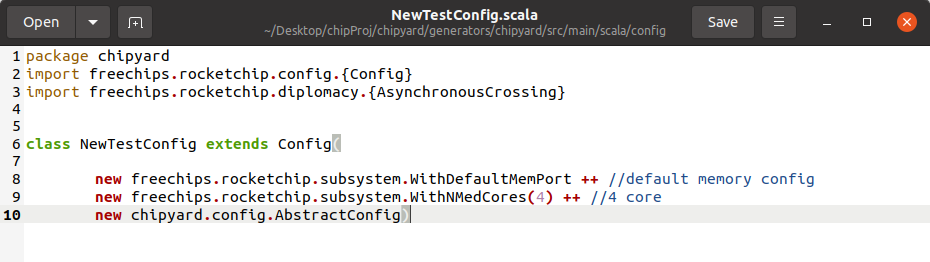
\includegraphics[width=0.7\linewidth]{NewTestConfig}
	\caption[]{NewTestConfig.scala}
	\label{fig:newtestconfig}
\end{figure}
	
\end{document}